\documentclass[12pt,a4paper,titlepage]{article}
\usepackage[utf8]{inputenc}
\usepackage{amsmath}
\usepackage{amsfonts}
\usepackage{graphicx}
\usepackage{amssymb}
\usepackage{setspace}
\usepackage{outlines}
\usepackage[title]{appendix}
\usepackage[round,authoryear]{natbib}
\graphicspath{{/Users/susanna/projects/sanitation/output/figures/}}
\newcommand\independent{\protect\mathpalette{\protect\independenT}{\perp}}
\def\independenT#1#2{\mathrel{\rlap{$#1#2$}\mkern2mu{#1#2}}}
\bibliographystyle{abbrvnat}
\usepackage[margin=1in]{geometry}
\author{Susanna Makela}
\title{The Causal Relationship between Sanitation and Child Height \\
		\Large Effects at Household and Community Levels}
\begin{document}
\maketitle
\singlespacing

\section{Introduction}
Height is an important measure of population health and human capital, with links to labor market outcomes \citep{case_paxson, vogl}, mortality \citep{jousilahti}, and cognitive achievement \citep{spears2012}. While genetics play a major role in determining maximum height, early life nutrition and disease environment strongly influence the extent to which this height potential is achieved \citep{humphrey}. One major determinant of the disease environment, particularly in less-developed countries, is exposure to poor sanitation in the form of open defecation. India has one of the highest rates of open defecation, with over 60\% of its rural population and 44\% of the overall population lacking toilet or latrine facilities in 2015 \citep{jmp_2015}.

India also has high rates of stunting, with 38\% of children in 2015 under the age of five being too short for their age \citep{nfhs4_factsheet}. Indeed, children in India are shorter, on average, than children in Africa, who are poorer, on average, and one proposed explanation for this ``Asian enigma'' is the high rates of open defecation in India \citep{spears_intl_variation}. Recent evidence in the form of a randomized field experiment \citep{village_san} and an ecological analysis at the district level \citep{ecological} suggests that there is a causal relationship between the sanitation environment at the neighborhood level and height-for-age among children in India. This study uses data from three household surveys to study the causal effects of open defecation at both the household and neighborhood levels in India using a sample of over 70,000 children from three rounds of a national household survey.

%\subsection{Sanitation and child health in India}
%Previous studies have established strong links between sanitation and child health in India, particularly at the neighborhood level. \cite{geruso_spears} estimate that a 10 percentage-point reduction in neighborhood-level open defecation ``is associated with a decline in infant mortality of 6.5 infants per 1,000''. Children in India tend to be exceptionally short for their height, particularly compared to children in sub-Saharan African countries, where children are poorer, on average; this puzzle is known as the ``Asian enigma'', and some studies suggest that open defecation, which is substantially more prevalent in India than in sub-Saharan Africa, can account for much of this discrepancy \citep{spears_intl_variation}. Within India, an ecological analysis at the district level \citep{spears_ecological} estimates that a 10 percentage-point increase in open defecation is associated with a 0.7 percentage point increase in stunting and severe stunting. A recent randomized field experiment in rural Maharashtra, India, that subsidized construction of household pit latrines and promotes sanitation at the village level yielded an increase of about 0.3 height-for-age standard deviations among children children under five after 18 months \citep{village_san}. This estimate is close to the 0.2 height-for-age standard deviation increase associated with the Total Sanitation Campaign, an Indian government program dedication to building latrines and promoting sanitation in India \citep{spears_tsc}.

\subsection{Causal questions}
In this study, we examine the effects of open defecation (hereafter OD) at the household and neighborhood levels on height for age of Indian children aged three and younger. Specifically, we ask and answer the following questions: (1) What is the effect of living in a household with a latrine in neighborhoods where the OD rate is low? (2) What is the effect of living in a household with a latrine in neighborhoods where the OD rate is high? (3) What is the effect of a high versus low neighborhood-level OD rate on children who are likely to live in a household with a latrine?

Note that we use the terms OD and latrine use interchangeably; a household practicing OD is assumed to not use a latrine or toilet, and vice versa. The first three of the above questions closely parallel those asked by \cite{hong_raudenbush} in a study of the effect of kindergarten retention on reading outcomes. We adopt their analytical framework for studying multilevel observational data as described in Section \ref{sec:framework} below.

\subsection{Data}
The data we use come from three rounds of the National Family Health Survey (NFHS). The NFHS is a cross-sectional survey conducted in 1992-93, 1998-99, and 2005-06 intended to yield estimates of indicators of maternal and child health, nutrition, and reproductive health valid for the rural and urban parts of Indian states. The NFHS includes anthropometric measurements of height for children born to interviewed mothers in the three years prior to the survey, as well as numerous mother- and household-level covariates. The outcome variable is the height-for-age $z$-score: a child's height converted into a $z$-score relative to the 2006 WHO healthy reference population. While children are naturally nested within mothers and households, we ignore this level of nesting in our analysis. Because heights are measured only for children born in the three years prior to the survey, 90\% of mothers and 89\% of households in our sample have data for only one child. Conversely, 81\% of the children in our sample are the only measured child of their mother and 89\% are the only measured child from their household.

For the purposes of this study, we define ``neighborhood'' to be the primary sampling unit (PSU) to which each household belongs. In rural areas, the PSUs are generally villages of up to 500 households (larger villages are split in two), and in urban areas the PSUs are census enumeration blocks (CEBs) consisting of 150-200 households (technically, the urban PSUs are census wards in which the CEBs are nested, but since one CEB is selected per ward, we can think of the CEB as the PSU \citep{roy_acharya}). Within selected PSUs, a sample of roughly 15-60 households is taken. To ensure adequate PSU-level sample sizes, we discard PSUs with fewer than 15 sampled households. We define OD at the household level as households reporting that their toilet facility is ``no facility/bush/field''. See Appendix \ref{sec:app_data} for more details on our sample.

%The NFHS, DLHS, and AHS all employ complex multi-stage sampling designs, with samples drawn separately in rural and urban areas. For the NFHS, villages are the primary sampling units (PSUs) in rural areas and are sampled with probability proportional to size (PPS). Villages with more than 500 households are split in two, and one of the groups is sampled using PPS. A simple random sample of households is then taken in the sampled villages. In urban areas, the PSUs are census wards, which are sampled using PPS sampling. A PPS sample of census enumeration blocks is taken in the selected wards; census enumeration blocks consist of roughly 150-200 households. Finally, a simple random sample of households is taken	 in the selected census enumeration blocks.

%While \cite{geruso_spears} suggest that there is little evidence for an interaction between household- and community-level open defecation; they found no difference in their causal estimates of the effect of neighborhood-level sanitation on infant mortality when estimated separately for households with and without latrines. Additionally, this claim was made in the context of infant mortality as the outcome. Mortality is much further down the causal chain from open defecation than is height for age. However, it may be that the interaction is actually operating at the neighborhood level. That is, it may be that household open defecation matters only in neighborhoods with low (or high) rates of open defecation. 


\section{Causal inference framework}\label{sec:framework}
\subsection{Relaxing SUTVA}
We use the potential outcomes framework of \cite{rubin1978} to define causal effects and the estimands. In a population of $N$ children, $i = 1, \ldots, N$, we let $z_i$ denote the treatment status of the household in which child $i$ lives: $z_i = 1$ if the household practices OD and $z_i = 0$ if it does not. We let $\mathbf{z} = (z_1, \ldots, z_N)$ denote the vector of treatment assignments for all $N$ children. Since the treatment is binary, $z_i \in \{0, 1\}$ and $\mathbf{z} \in \{0, 1\}^{2N}$. The potential outcome of child $i$, were their household's treatment status $z_i$ and the other households' treatments $\mathbf{z}_{-i} = (z_1, \ldots, z_{i-1}, z_{i+1}, \ldots, z_N)$, is $Y_i(\mathbf{z})$.

A fundamental assumption that makes causal identification possible in the potential outcomes framework is the stable unit treatment value assumption (SUTVA). SUTVA states that there is a single version of the treatment and that the potential outcome of one unit is independent of the treatment assignment of the other units \citep{rubin1986}. In other words, SUTVA allows us to simplify the definition of potential outcome and write $Y_i(\mathbf{z}) \equiv Y_i(z_i, \mathbf{z}_{-i}) = Y_i(z_i)$. In our context, SUTVA implies that the potential outcome for a child depends only on the sanitation status of their own household and not on that of their neighbors.

A key methodological challenge in this study is that SUTVA is an unreasonable assumption. Because OD by definition occurs outdoors, the practice of OD by one household necessarily exposes others in the neighborhood to possible contact with human waste. It is therefore entirely plausible that the sanitation behavior of the neighbors of a given household can affect the potential outcome of a child in that household, regardless of the sanitation status of that household.

Our analytical strategy for relaxing SUTVA is inspired by the approach taken by \cite{hong_raudenbush}, hereafter HR, in a study of the causal effect of kindergarten retention (i.e. repeating kindergarten) on reading outcomes, a context in which SUTVA is also an implausible assumption. \cite{hong_raudenbush} handle this complication by assuming that the collective effects of $\mathbf{z}_{-i}$ on $Y_i(\mathbf{z})$ can be summarized by $z_i$ and a scalar function $v(\mathbf{z})$, so that
\begin{equation}\label{eq:hr_pot_out}
	Y_i(\mathbf{z}) \equiv Y_i(z_i, \mathbf{z}_{-i}) = Y_i(z_i, v(\mathbf{z})).
\end{equation}
Following HR, we use $v(\mathbf{Z}) = V$ to denote the binary random variable representing the neighborhood-level OD rate that takes on values $v(\mathbf{z}) = v = 0$ in low-OD neighborhoods and $v(\mathbf{z}) = v = 1$ in high-OD neighborhoods. Empirically, we use the average OD rate by survey round and rural-urban status to classify neighborhoods as high- or low-OD. See Appendix \ref{sec:app_data} for details.

Given two sets of possible treatment assignments for a single unit and all units, $(z, \mathbf{z})$ and $(z^{\prime}, \mathbf{z}^{\prime})$, a generic causal estimand is of the form $\mathbb{E}[Y(z, v(\mathbf{z})) - Y(z^{\prime}, v(\mathbf{z}^{\prime}))]$. This formulation relies on three main assumptions as described by HR: a) causal inferences are generalized conditional on current neighborhood residence; b) there is no interference between neighborhoods, and c) treatment assignment at both the household and neighborhood levels are strongly ignorable conditional on observed covariates. See Appendix \ref{sec:assumptions} for a more detailed description of these assumptions.

\subsection{Subpopulations and estimable causal quantities}
An important feature of HR's analysis of kindergarten retention rates is their division of children into subpopulations depending on their risks of retention under high and low school-level retention rates. They make this division because some potential outcomes are not defined for some children: some children may only be retained under a high school-level retention rate but not under a low one, while other may never be retained regardless of the school-level rate.

The identification of subpopulations is relevant in our context as well. In rural north India, notions of purity, pollution, caste, and religion play an integral role in deep-seated sanitation preferences that make ending OD particularly challenging \citep{squat, san_culture}. OD rates in India as a whole are starkly different by both rural vs.\ urban residency and by religion. Data from NFHS-3 in 2005-06 show that 17\% of urban households practiced OD, compared to 74\% of rural households. The same data also show that nearly 60\% of Hindu households practiced OD, while only 40\% of the relatively poorer Muslim households did.

Let $q_1$ denote the probability of a household practicing OD under a high neighborhood OD rate and $q_0$ denote the probability under a low rate. Assume that $q_1 \geq q_0$ for all households. In parallel with HR, we identify three subpopulations of households (equivalently, children, as we ignore the clustering of children in households):
\begin{itemize}
	\item[(A)] Households at risk of OD under a low neighborhood OD rate ($q_1 \geq q_0 > 0$)
	\item[(B)] Households at risk of OD under a high neighborhood OD rate but not a low rate ($q_1 \geq q_0 = 0$)
	\item[(C)] Households at no risk even under a high neighborhood OD rate ($q_1 = q_0 = 0$)
\end{itemize}
See Table \ref{table:1} of Appendix \ref{sec:estimands} for more details on the potential outcomes and causal effects defined for these subpopulations.

Because of the observational nature of our data, only certain causal quantities are estimable. Specifically, our estimands parallel those in HR and are as follows (see Appendix \ref{sec:estimands} for details). First, we estimate the conditional effect of household OD for children in subpopulation (A) who live in low-OD neighborhoods,
\begin{equation}\label{eq:delta_z0}
	\delta_{Z0} = \mathbb{E}[Y_A(1,0) - Y_A(0,0) \mid V=0, \mathbf{X}, \mathbf{W}],
\end{equation}
where $\mathbf{X}$ and $\mathbf{W}$ are child- and neighborhood-level covariates, respectively. Second, we consider the union of subpopulations (A) and (B), which we denote (AB). Children in subpopulation (AB) are those who are ever at risk for living in households that practice OD ($q_1 > 0$). For this ever-at-risk subpopulation, we estimate the conditional effect of household OD in high-OD neighborhoods for children actually living in high-OD neighborhoods:
\begin{equation}\label{eq:delta_z1}
	\delta_{Z1} = \mathbb{E}[Y_{AB}(1,1) - Y_{AB}(0,1) \mid V=1, \mathbf{X}, \mathbf{W}].
\end{equation}
The third estimand is the average causal effect of high vs.\ low neighborhood OD level for children in subpopulation (C), that is, the effect of neighborhood OD for children at no risk of living in households that practice OD:
\begin{equation}\label{eq:delta_v0}
	\delta_{V0} = \mathbb{E}[Y_C(1,1) - Y_C(0,1) \mid V=0, \mathbf{W}].
\end{equation}

\section{Estimation and inference}
\subsection{Propensity scores}
We follow HR in using propensity score stratification to estimate the causal effects $\delta_{Z0}$, $\delta_{Z1}$, and $\delta_{V0}$. We estimate propensity scores at two levels. First, we use logistic regression to estimate the neighborhood-level propensity for a high OD rate conditional on observed neighborhood covariates:
\[
	Q = \mathbb{P}(V=1 \mid \mathbf{W}).
\]

We then estimate $q_1$ and $q_0$, the propensities for household-level OD for households in high- and low-OD neighborhoods, respectively, and use them to identify subpopulations (A), (B), and (C); see Appendix \ref{sec:ps_models} for details. We use \texttt{R} and the \texttt{Rstan} package for all analyses.

\subsection{Causal effects}
In \eqref{eq:delta_z0}, we defined $\delta_{Z0}$, the causal effect of being in an OD household in a low-OD neighborhood. Given the assumptions outlined above and in the appendices, we can condition on $q_0$ in place of $\mathbf{X}$ and $\mathbf{W}$, and \eqref{eq:delta_z0} is thus equivalent to
\[
	\delta_{Z0} = \mathbb{E}[Y_A(1,0) - Y_A(0,0) \mid V=0, q_0].
\]
To estimate $\delta_{Z0}$, we use a hierarchical linear regression similar to the approach taken by HR:
\begin{align*}
	Y_i &\sim N \left( \beta_0 + u_{j[i]} + (\delta_{Z0} + \Delta_{Z0j[i]})z_i + \sum_{g=1}^G \beta_g q_{0gi} + \beta_9 ~ \text{logit}(\widehat{q_{0i}}), \sigma^2 \right) \\
	\begin{pmatrix}
	  u_j \\
	  \Delta_{Z0j}
	\end{pmatrix} &\sim N \left[ \begin{pmatrix}
         	                       0 \\
         	                       0
	                             \end{pmatrix}, \begin{pmatrix}
	                                              \tau_u & \tau_{u \cdot Z_0} \\
	                                              \tau_{u \cdot Z_0} & \tau_{Z0}
	                                            \end{pmatrix} \right].
\end{align*}
Here $i$ indexes households/children, $j$ indexes neighborhoods and $j[i]$ denotes the neighborhood to which household $i$ belongs. The outcome $Y_i$ is the height-for-age $z$-score, $z_i$ is the household-level OD indicator, and $q_{0gi}$, $g = 1, \ldots, G$ are indicators for the $G=10$ strata of $q_0$. Following HR, we also include the estimate $\widehat{q}_{0i}$ on the logit scale for additional bias reduction. Here $u_j$ is a neighborhood-level random intercept that captures baseline differences in height-for-age across neighborhoods, while $\Delta_{Z0j}$ is the neighborhood-level variation in the treatment effect. Neighborhood variation in the household-level treatment effect is captured by $\tau_{Z0}$, and we can also estimate the covariance between $\Delta_{Z0j}$ and $u_j$ with $\tau_{u \cdot Z_0}$.

Among children in low OD neighborhoods, the adjusted within-stratum difference in means of height-for-age $z$-scores between children in OD and non-OD households is $\widehat{\delta}_{Z0} = -0.17$ (SE 0.03). This household-level OD effect varied across neighborhoods, with $\widehat{\tau}_{Z0} = 0.73$. If $\Delta_{Z0j}$ really were normally distributed, then we would expect 95\% of the household-level OD effects to range from -1.60 to 1.27 ($\widehat{\delta}_{Z0} \pm 1.96 \widehat{\tau}_{Z0}$) in low-OD neighborhoods. 

Similarly, our definition of $\delta_{Z1}$ given in \eqref{eq:delta_z1} is equivalent to
\[
	\delta_{Z1} = \mathbb{E}[Y_{AB}(1,1) - Y_{AB}(0,1) \mid V=1, q_1].
\]
We use a model analogous to the one above, restricting ourselves to children in subpopulation (AB) -- that is, those for whom we estimate $q_1 > 0$. For children in subpopulation (AB) who are at risk of living in OD households in high-OD neighborhoods, the estimated treatment effect is $\widehat{\delta}_{Z1} = -0.18$ (SE 0.02). Here again we observe significant variation across neighborhoods, with $\widehat{\tau}_{Z1} = 0.71$, which would lead to a 95\% range of -1.56 to 1.21 for household-level OD effects in high-OD neighborhoods. This is quite similar to the case for low-OD neighborhoods, suggesting that the effect of household-level OD does not vary much by (binary) neighborhood OD level.

For estimating $\delta_{V0}$, we use children in subpopulation (C) for whom we estimate $q_1 = 0 = q_0$. Our hierarchical model in this case is
\begin{align*}
	Y_i &\sim N \left( \beta_0 + u_{j[i]} + \delta_{V0} v_j + \sum_{h=1}^H \beta_h Q_{hj} + \beta_9 ~ \text{logit}(\widehat{Q_{j}}), \sigma^2 \right) \\
	u_j &\sim N(0, \tau),
\end{align*}
where $v_j$ denotes the neighborhood OD level and $Q_{hj}$ are indicators for the $H=10$ strata of $\widehat{Q_j}$. We estimate that the neighborhood-level effect of high vs low OD levels among children not at risk of living in OD households is $\delta_{V0} = 0.98$ (SE 0.67). This estimate is not statistically significant, meaning we cannot detect an effect of high vs low OD neighborhoods on height-for-age among children at low risk of living in OD households.

%
%since the effect of retention on a particular child could be affected by the retention status of other children, as well as the overall retention rate of the child's school. By making the assumption that conditioning on propensity scores of treatment at both the school and student levels render the assignment mechanism strongly ignorable, the authors treat their observational data as approximating a two-stage randomized experiment. This assumption, coupled with stratifying on the multilevel propensity score, allows them to estimate several causal quantities of interest: the effect of retention in high-retention schools and low-retention schools, and the effect of a high retention rate compared to a low retention rate.

%We follow this overall approach, but while \cite{hong_raudenbush} assume that treatment assignments at both the group (school) and unit (student) levels are binary, we take an approach that allows the group-level treatment assignment to be continuous by using the generalized propensity score (GPS).
%
%The GPS was proposed in parallel work by \cite{imai_vandyk} and \cite{hirano_imbens}. The *brief discussion of GPS here*.
%
%Several methods exist for estimating the GPS \citep{imai_vandyk,hirano_imbens}. Recent studies have advocated using machine learning methods including boosting \citep{zhu_etal} and Super Learners \citep{kreif_etal}. However, as noted by \cite{kluve_etal}, the exact form of the GPS model is less important than the degree to which any given model balances the distribution of observed covariates for a given value or stratum of treatment. 
%
%
%In attempting to estimate the effects of OD operating at both the household and neighborhood levels, we are entering a situation in which the stable unit treatment value assumption (SUTVA) is implausible. If we consider the OD status of a household as a binary treatment, it is clear that the potential outcome for a child is likely to be affected by the OD status of other households in their neighborhood, as the amount of fecal matter they are exposed to depends not only on their own household, but their overall environment. Let $Z_i$ denote the treatment to which child $i$ is exposed: treatment $Z_i = 0$ if they live in a household that does not practice OD and $Z_i = 1$ if they do. The potential outcome for child $i$ is then $Y_i(\mathbf{Z}_j)$, where $\mathbf{Z}_j = \{Z_i: i \in village_j\}$. SUTVA allows us to write $Y_i(\mathbf{Z}_j) = Y_i(Z_i)$, but 
%
%The OD status of adjacent households can affect a child's potential outcomes, as can the community's overall OD rate, as it may affect water/food quality (?), exposure of the child to fecal matter via their mother and other household members who move through the community.
%
%Recent work has considered implications of relaxing SUTVA in experimental contexts (cite that guy who presented this fall?), as well as in network causal inference, where it by definition doesn't hold (cite some network stuff here?). Because our data are a random sample of households in the community and do not include geographic detail beyond anonymized PSU identifiers, we have no way of knowing the geographic adjacencies between households in the community. It's also difficult to think about the causal effect of one specific household changing their OD status on another household, and it's not that interesting. Instead, this study asks about the causal effect of household-level OD at a given community OD level, and about the community-level OD effect for a fixed household OD status. In order to account for the interference present in our data, we follow \cite{hong_raudenbush} and make the identifying assumption that the effect of other households' OD status can be summarized through a scalar function $r(\mathbf{Z}_j)$:
%\[
%	Y_i(\mathbf{Z}_j) \equiv Y_i(Z_i, \mathbf{Z}_{-i,j}) = Y_i(Z_i, r(\mathbf{Z}_j)).
%\]
%
%In contrast to \cite{hong_raudenbush}, we do not make the further simplification of setting $r(\mathbf{Z}_j) = 1$ for high-OD communities and $r(\mathbf{Z}_j) = 0$ for low-OD communities. Instead, we allow $r(\mathbf{Z}_j)$ to take on values in $[0, 1]$.
%
%Following \cite{hong_raudenbush}, we make three additional assumptions. First, because we would like to generalize our results to the entire population of communities as they currently exist in India and not communities formed by randomly assigning people to live in them, we treat communities as ``intact''. That is, we will estimate average treatment effects conditional on current community membership. Second, we assume there is no interference between communities. While we allow for interference between households in the same community via the GPS, we assume the potential outcomes of children in a given community are independent of treatment assignment of households in other communities. Finally, we assume that treatment assignment at both the household and community levels are (strongly) ignorable conditional on the observed community- and household-level covariates.
%

%\subsection{Generalized propensity score}
%\subsubsection{Framework}
%Methods for generalizing propensity scores for nonbinary treatments have been developed by \cite{imai_vandyk} and \cite{hirano_imbens}. In contrast to the propensity score developed by \cite{rosenbaum_rubin}, which assumes a binary treatment, these generalizations allow for the treatment to be categorical, ordinal, continuous, or even multivariate \citep{imai_vandyk}. We follow the approach of \cite{hirano_imbens} that defines the generalized propensity score and describing its properties for a continuous treatment.
%
%We briefly describe the generalized propensity score (GPS) as developed by \cite{hirano_imbens}, closely following their presentation. We have $N$ units, $i = 1, \ldots, N$, each assigned a treatment $t$ that takes values in $\mathcal{T}$. For a binary treatment, $\mathcal{T} = \{0, 1\}$, but for our purposes we take $\mathcal{T} = [0, 1]$. Our goal is to estimate the average dose-response function (DRF)
%\begin{equation}\label{eq:drf}
%	\mu(t) = \mathbb{E}[Y(t)].
%\end{equation}
%
%In parallel with the binary treatment case, the utility of the GPS depends on several assumptions. First, we assume that treatment is weakly unconfounded conditional on observed covariates $X$, so that
%\[
%	Y(t) ~\perp~ T \mid X \quad \text{for all} ~ t \in \mathcal{T}.
%\]
%Here the term ``weak'' refers to the fact that we do not require joint independence of all potential outcome $\{Y(t)\}_{t \in \mathcal{T}}$. Let $r(t,x) = f_{T \mid X}(t \mid x)$ denote the conditional density of the treatment given the covariates. The GPS is then this conditional density evaluated at the observed values of $T$ and $X$:
%\begin{equation}\label{eq:gps}
%	R = r(T, X).
%\end{equation}
%In practice, the GPS can be estimated with any parametric or nonparametric method. A simple example is a linear regression of $T$ on $X$: $T_i \mid X_i \sim N(\beta_0 + \beta_1^T X_i, \sigma^2)$. Recent studies have explored machine learning approaches like Super Learners \citep{kreif_etal} and boosting \citep{zhu_etal}. However, as \cite{kluve_etal} point out, the primary concern with modeling the GPS is that it achieves adequate covariate balance; just as with the propensity score for a binary treatment, the specific modeling approach is less important than obtaining scores that yield balance on the observed covariates.
%
%As \cite{hirano_imbens} describe, a mechanical property of the GPS endow it with a balancing property, namely that within strata defined by $r(t, X)$, the probability that $T=t$ is independent of $X$: $X ~\perp~ \mathbf{T=t} \mid r(t, X)$. This mechanical property does not require unconfoundedness. However, in conjunction with weak unconfoundedness, this property implies that treatment assignment is unconfounded conditional on the GPS:
%\begin{equation}\label{eq:gps_unconf}
%	Y(t) ~\perp~ T \mid r(t, X).
%\end{equation}
%In other words, we need no longer condition on the (likely high-dimensional) covariate $X$ to achieve unconfoundedness of the treatment; conditioning on the GPS is sufficient.
%
%We can now use the GPS to obtain an unbiased estimate of the DRF $\mu(t)$. The first step is to estimate the conditional expectation of the outcome given the treatment and the GPS,
%\begin{equation}\label{eq:beta}
%	\beta(t,r) = \mathbb{E}[Y \mid T=t, R=r].
%\end{equation}
%This step requires us to specify a model for $Y$ as a function of $T$ and $R$. \cite{hirano_imbens} proposed a linear regression of $Y$ on $T$ and $R$ with  quadratic terms:
%\[
%	Y_i \mid T_i, R_i \sim N(\alpha_0 + \alpha_1 T_i + \alpha_2 T_i^2 + \alpha_3 R_i + \alpha_4 R_i^2 + \alpha_5 T_i R_i, \sigma^2),
%\]
%Of course, more flexible nonparametric models can also be used; recent studies have employed splines \citep{zhu_etal} and Super Learners \citep{kreif_etal}. Whatever the model we choose, the estimation is done using the observed $T_i$ and estimated $\widehat{R}_i = \widehat{r}(T_i, X_i)$ for each individual.  As \cite{hirano_imbens} emphasize, $\beta(t,r)$ does not have a causal interpretation.
%
%The second step is to estimate the DRF itself, $\mu(t) = \mathbb{E}[\beta(t,r)]$, where the expectation is taken over the GPS evaluated at the treatment level of interest $t$ and observed covariates $X$, $r(t, X)$. With an estimate of $\mu(t)$ in hand, we can calculate the causal effect of dose $t$ relative to a baseline or control dose $t^{\prime}$, $\mathbb{E}[Y(t)-Y(t^{\prime})]$, or the marginal treatment effect function $d\mu / dt$. In practice, we estimate $\mu(t)$ as
%\[
%	\widehat{\mu}(t) = \frac{1}{N} \sum_{i=1}^N \beta_i(t, \widehat{r}(t, X_i))
%\]
%
%\subsubsection{Multilevel treatments}
%The main methodological contribution of this study is combining use of the GPS for continuous treatments \citep{hirano_imbens} with the framework that allows us to view an observational study as an approximation of a two-stage experiment \citep{hong_raudenbush}. 
%
%
%
%\subsubsection{Implementation}
%
%We have a sample of $i = 1, \ldots, n$ units and a treatment $t$ taking values in the interval $[t_0, t_1]$. The potential outcome for unit $i$, were they to receive treatment $t$, is $Y_i(t)$. In contrast to the case with a binary treatment, where our goal is to estimate the average treatment effect $ATE = \mathbb{E}[Y_i(1) - Y(_i0)]$, our goal here is to estimate the average dose-response function $\mu(t) = \mathbb{E}[Y_i(t)]$. We observe a $p \times 1$ vector of covariates $\mathbf{X}_i$ for each unit $i$, and assume weak unconfoundedness of the potential outcomes and treatment conditional on the covariates:
%\[
%	Y(t) \independent T \mid X, \quad \text{for all}~ t \in [t_0, t_1].
%\]
%
%Define $r(t, x)$ to be the conditional density of the treatment at a particular value of the covariate vector:
%\[
%	r(t, x) = f_{T \mid X}(t \mid x).
%\]
%The GPS is then $R = r(T, X)$. The assumption of weak unconfoundedness above implies that
%\[
%	f(t \mid Y(t), \mathbf{X}) = f(t \mid \mathbf{X}) \quad \text{for all}~ t \in [t_0, t_1].
%\]
%As \cite{hirano_imbens} show, the GPS is a balancing score in a manner similar to that of the propensity score, and this property combined with unconfoundedness means that treatment assignment is unconfounded given only the GPS:
%\[
%	f_T (t \mid Y(t), \mathbf{X}, r(t, \mathbf{X})) = f_T (t \mid Y(t), r(t, \mathbf{X})) = f_T (t \mid r(t, \mathbf{X})).
%\]

%PSU-level covariates
%\begin{enumerate}
%	\item Avg asset ownership
%	\item Prop HH's with electricity
%	\item Prop HH's with improved water
%	\item Prop HH's Muslim
%	\item Prop institutional delivery
%	\item Prop w/ health card
%	\item Prop w/ mother literate
%	\item Prop w/ child ever vaccinated
%\end{enumerate}



%Outline
%\begin{itemize}
%	\item Approximation of an observational study as a two-stage randomized experiment
%	\item Continuous treatment on the PSU level -- apply Imai/van Dyk and/or Hirano/Imbens methods for dealing with generalized propensity scores to estimate the PSU-level generalized propensity score
%	\item Multilevel observational study
%\end{itemize}

%\section*{Data}
%The data we use come from the first three rounds of the National Family Health Survey (NFHS), a household survey designed to yield estimates of important indicators of maternal and child health for all 29 Indian states by rural/urban residence. The three rounds took place in 1992-1993, 1998-1999, and 2005-2006. We use the household questionnaire to determine whether the household practices open defecation, other important household characteristics (asset ownership, access to an improved water source, electricity, housing material), and also to calculate PSU-level OD rates. Our outcome is an age-and-sex-standardized measure of height-for-age for children born in the three years prior to the survey. We have data on a total of XXX children over the three survey rounds.

%; a fourth round was completed in 2015-2016, but those data are yet to be made public. The NFHS uses a multi-stage sampling design, with samples drawn separately in rural and urban areas. In rural areas, villages are the primary sampling units (PSUs), and are sampled with probability proportional to size (PPS). A simple random sample of households is then taken in the sampled villages. In urban areas, the PSUs are census wards, which are sampled using PPS sampling. A PPS sample of census enumeration blocks is taken in the selected wards, followed by a simple random sample of households in the selected census enumeration blocks.

%The NFHS includes multiple questionnaires. We use the household questionnaire, administered to the head of the household, and the women's questionnaire, administered to eligible women of reproductive age. Eligibility has varied across the three rounds, so we use data collected for ever-married women ages 15-49, a group that is considered eligible in each round. The women's questionnaire includes detailed information on the children born in the last several years prior to the survey, including vaccination history, nutritional status, recent illnesses, and anthropometry measurements. Because the 



%- NFHS1-3
%- DLHS???
%- 
%
%We can't use \% Muslim as in IV the way Spears et al did, because when we plot various indicators (\% with improved water, \% with latrine, \% asset ownership, \% with electricity) against \% Muslim, we do NOT see the same pattern they did. This is probably because we separate the plots by survey round, while they combine them. This holds even when we exclude PSUs with 0\% and 100\% Muslim populations. So it does not seem to hold that \% Muslim is correlated with predictors of worse child health, except for sanitation.
%
%In this case, we need another way of getting at the causal effect of neighborhood sanitation. One thing we could do is match children with similar household/mother/child characteristics across PSUs with different sanitation levels. This would help approximate the randomized experiment where otherwise similar children/households are randomly assigned to different levels of sanitation. The key would be to be able to find suitable matches -- 
%
%
%Suppose we were only interested in estimating the household-level effect of sanitation. Then we could estimate the propensity score for having a toilet and match on this propensity score. I guess here could just ignore the neighborhood effect?
%
%Notation. Let $i$ index households, $j$ index PSUs, $t$ index survey round. $T_{ijt}$ is a binary treatment variable denoting whether household $i$ in PSU $j$ in survey round $t$ practices OD. The outcome is $Y_{ijt}$, the height-for-age $z$-score for a child (here we ignore the fact that children are actually nested in households). If matching on $e(x) = Pr(T_{ijt} = 1 \mid X_{ijt} = x)$ sufficiently balances potential confounders $X_{ijt}$ between treatment and control groups, then we can be more confident that our estimates of treatment effect are unbiased.


%
%\begin{itemize}
%	\item Pair matching PSUs that are far apart in terms of prop Muslim -- ``stronger'' IV?
%	\item OR pair-matching kids with different HH sanitation status across similar prop Muslim/prop OD PSUs -- this could get at the HH-leve effect?
%	\item Can we somehow formulate this as an observational version of the Imai et al matched-pair cluster-randomization idea?
%\end{itemize}
%
%Suppose sanitation level were randomly assigned across clusters. Then, we could estimate the causal effect of cluster-level sanitation on individual children. 
%
%We match children in households that practice OD with children in households that do not. We exactly match for NFHS round, state, rural/urban, whether the household has an improved water source, the religion of the household head (Hindu/Muslim/Other), and whether the mother is literate. We also balance the means of the proportion of the nine assets that a household has, whether the mother lives with her in-laws, and the age of the mother at the time of the interview.

\section{Discussion}
Given the stubbornly high rates of OD in India and the growing evidence of the causal relationship between sanitation and health, further research into the specific causal mechanisms of how sanitation affects height is urgently needed. Specifically, research on potential effect modifiers and variability in the treatment effect of OD at both household and neighborhood levels will enable policymakers to better target resources into expanding latrine use and mitigating the negative effects of OD.

While observed neighborhood OD rates are naturally continuous over $[0,1]$, we have dichotomized them into low and high, perhaps unnecessarily throwing away some information. A better approach might be to extend the framework of HR to allow the neighborhood rate to vary continuously from 0 to 1. Such an extension would require the use of the generalized propensity score \citep{hirano_imbens}, which extends the propensity score and its balancing properties to nonbinary treatments to estimate the neighborhood OD propensity $Q$.

See Appendix \ref{sec:lims} for a discussion of the limitations of this study.


\bibliography{sanitation}

%%%%%%%%%%%%%%%%%%%%%%%%%%%%%%%%%%%%%%%%%%%%%%%%%%%%%%%%%%%%%%%%%%%%%%%%%%%%%%%%%%%%%%%%%%%%%%%%%%%%%%%%%%%%%%%%%%%%%%%%%%%%%%%
%%%%%%%%%%%%%%%%%%%%%%%%%%%%%%%%%%%%%%%%%%%%%%%%%%%%% APPENDICES %%%%%%%%%%%%%%%%%%%%%%%%%%%%%%%%%%%%%%%%%%%%%%%%%%%%%%%%%%%%%%
%%%%%%%%%%%%%%%%%%%%%%%%%%%%%%%%%%%%%%%%%%%%%%%%%%%%%%%%%%%%%%%%%%%%%%%%%%%%%%%%%%%%%%%%%%%%%%%%%%%%%%%%%%%%%%%%%%%%%%%%%%%%%%%


\begin{appendices}

\section{NFHS data}\label{sec:app_data}
Figure \ref{fig:zlen} shows the distribution of height-for-age $z$-scores by survey round and household OD status. Height is measured for children born in the three years prior to the survey to ever-married women aged 15-49. The $z$-scores are calculated relative to the 2006 WHO reference population and are adjusted for age and sex. Extreme values of the $z$-scores ($|z|>6$), likely resulting from measurement and/or transcription error, have been dropped. Table \ref{table:ss} displays the sample size by survey round.

\begin{figure}[h!]\label{fig:zlen}
	\centering
	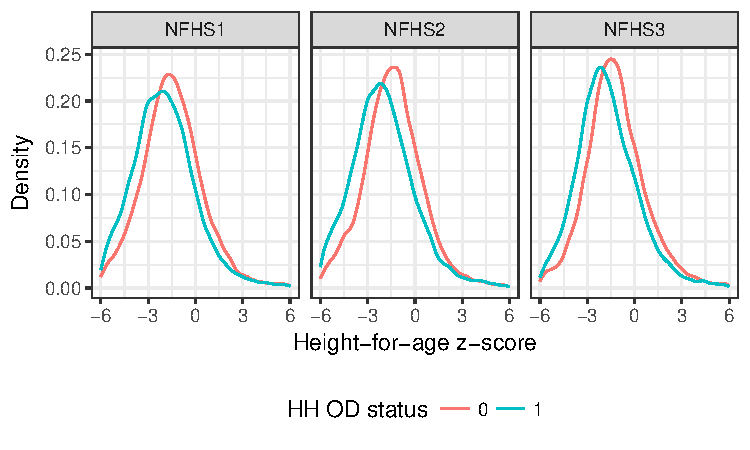
\includegraphics[scale=1]{zlen_density.pdf}
	\caption{Distribution of height-for-age $z$-scores by survey round and household OD status.}
\end{figure}

\begin{table}[ht]
\centering
\begin{tabular}{rr}
  \hline
 Round & N \\ 
  \hline
NFHS1 & 20993 \\ 
  NFHS2 & 25727 \\ 
  NFHS3 & 24896 \\ 
   \hline
\end{tabular}
\caption{Sample size by survey round.}
\label{table:ss}
\end{table}

Table \ref{table:nfhs_od} displays the OD rates by survey round and rural-urban residence, with rates for all India shown for reference. NFHS-1 was conducted in 1992-93, NFHS-2 in 1998-99, and NFHS-3 in 2005-06.

\begin{table}[h!]
	\small
	\centering
	\begin{tabular}{lccc}
		  & NFHS-1 & NFHS-2 & NFHS-3 \\
		 \hline
		 Rural & 87.1 & 80.8 & 74.0 \\
		 Urban & 24.1 & 19.2 & 16.8 \\
		 All India & 69.7 & 63.7 & 55.4 \\
		 \hline
	\end{tabular}
	\caption{OD rates (\%) by survey round and rural-urban residency.}
	\label{table:nfhs_od}
\end{table}

\begin{figure}[h!]\label{fig:psu_od_dist}
	\centering
	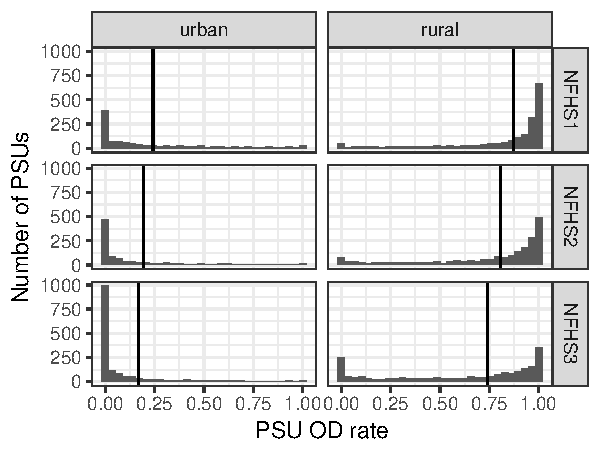
\includegraphics[scale=1]{psu_od_rate_hist.pdf}
	\caption{PSU (neighborhood) OD rates by survey round and rural-urban residency. Vertical lines denote mean OD rate. Only PSUs with at least 15 sampled households are included.}
\end{figure}


\section{Causal assumptions}\label{sec:assumptions}
In this section, we provide details on the main assumptions underlying our causal framework as established by \cite{hong_raudenbush}.
	
\textit{Intact neighborhoods.} The generic estimand above implicitly ignores the assignment of individuals to neighborhoods. If we were to take this assignment into account, we would include the vector of neighborhood assignments $\mathbf{s}$ in the potential outcome, where $\mathbf{s} = (s_1, \ldots, s_N)$ and $s_i \in \{1, \ldots, J\}$ denotes which of the $J$ neighborhoods unit $i$ is assigned to. The estimand would then be
\[
	\mathbb{E}[Y(z, \mathbf{z}, \mathbf{s}) - Y(z^{\prime}, \mathbf{z}^{\prime}, \mathbf{s}^{\prime})],
\]
where $\mathbf{s}$ and $\mathbf{s}^{\prime}$ are two vectors of possible neighborhood assignments. However, we know that in the real world, people are not assigned to neighborhoods at random, and we wish to estimate causal effects conditional on actual neighborhood membership. We therefore condition our estimands on the observed neighborhood assignment $\mathbf{s}^*$:
\[
	\mathbb{E}[Y(z, \mathbf{z}, \mathbf{s}^*) - Y(z^{\prime}, \mathbf{z}^{\prime}, \mathbf{s}^*) \mid \mathbf{S} = \mathbf{s}^*].
\]
For clarity of notation, we consider all estimands to be conditional on $\mathbf{S} = \mathbf{s}^*$ from this point forward and do not explicitly write out this conditioning.

\textit{No interference between neighborhoods.} We assume that the potential outcome for a child can be affected by the treatment assignments of other children in the same neighborhood, but not by the treatment assignments of children from other neighborhoods. We therefore write $\mathbf{z}_j = (z_{1j}, \ldots, z_{n_j j})$ for the vector of treatment assignments for the $n_j$ children in neighborhood $j$ and $\mathbf{s}_j = (j, \ldots, j)$ for the corresponding neighborhood assignments. The potential outcome for a child is then
\[
	Y_i(z_i, v(\mathbf{z}), \mathbf{s}^*) = Y_i(z_i, v(\mathbf{v}_{j[i]}), \mathbf{s}_{j[i]}^*) \equiv Y_i(z_i, v),
\]
where the notation $j[i]$ refers to the neighborhood $j$ that unit $i$ belongs to. We let $V = v(\mathbf{Z})$ denote the random variable taking on values $v(\mathbf{z}) = v \in [0, 1]$.

\textit{Strongly ignorable treatment assignment.} We assume that the assignments of intact neighborhoods to open defecation level $V=v$ and children to household latrine use status $Z=z$ are ignorable conditional on observed neighborhood-level covariates $\mathbf{W}$ and child- and household-level covariates $\mathbf{X}$. Under this assumption, we can write
\[
	\mathbb{E}[Y(z,v) \mid Z=z, V=v, \mathbf{X} = \mathbf{x}, \mathbf{W} = \mathbf{w}] = \mathbb{E}[Y(z,v) \mid \mathbf{X} = \mathbf{x}, \mathbf{W} = \mathbf{w}],
\]
allowing us to estimate the conditional average causal effect
\[
	\mathbb{E}[Y(z,v) \mid \mathbf{X} = \mathbf{x}, \mathbf{W} = \mathbf{w}] - \mathbb{E}[Y(z^{\prime},v^{\prime}) \mid \mathbf{X} = \mathbf{x}, \mathbf{W} = \mathbf{w}]
\]
with the observed quantity
\[
	\mathbb{E}[Y(z,v) \mid Z=z, V=v, \mathbf{X} = \mathbf{x}, \mathbf{W} = \mathbf{w}] - \mathbb{E}[Y(z^{\prime},v^{\prime}) \mid Z=z^{\prime}, V=v^{\prime}, \mathbf{X} = \mathbf{x}, \mathbf{W} = \mathbf{w}]
\]

Together, the assumptions of intact neighborhoods, no interference between neighborhoods, and strong ignorability allow us to conceive of our observational data as approximating a two-stage experiment. In the first stage, neighborhoods are randomly assigned an open defecation rate within blocks defined by $\mathbf{W}$. In the second stage, households within neighborhoods are randomly assigned to binary latrine use within blocks defined by $\mathbf{X}$ and $\mathbf{W}$.
%We briefly describe these three assumptions and then give more detail on this approximation.

\section{Causal estimands and strong ignorability}\label{sec:estimands}
Table \ref{table:1} displays the potential outcomes and causal effects of interest for subpopulations of households defined by their probabilities of OD under high and low neighborhood-level OD rates. This table parallels Table 2 of HR.

\begin{table}[h!]
	\small
	\centering
	\begin{tabular}{cccc}
		 Subpopulation & Probabilities of OD & Potential outcomes & Causal effects of interest \\
		 \hline
		 (A) & $q_1 \geq q_0 > 0$ & $Y(1,1), Y(0,1), Y(1,0), Y(0,0)$ & $\mathbb{E}[Y(1,1) - Y(0,1)]$ \\
		     &  &  & $\mathbb{E}[Y(1,0) - Y(0,0)]$ \\
		 (B) & $q_1 \geq q_0 = 0$ & $Y(1,1), Y(0,1)$ & $\mathbb{E}[Y(1,1)-Y(0,1)]$ \\ 
		 (C) & $q_1 = q_0 = 0$ & $Y(0,1), Y(0,0)$ & $\mathbb{E}[Y(0,1)-Y(0,0)]$ \\ 
		 \hline
	\end{tabular}
	\caption{Potential outcomes and causal effects for subpopulations of households}
	\label{table:1}
\end{table}

To understand which causal effects are estimable under strong ignorability, we imagine that our observational data are in fact from two-stage randomized experiment. Neighborhoods are first randomized to a binary OD level $V = v \in \{0,1\}$ within blocks defined by neighborhood covariates $\mathbf{W}$ with probability $Q = Q(\mathbf{W})$: 
\begin{equation}\label{eq:Q_def}
	Q = \mathbb{P}(V=v \mid \mathbf{W}).
\end{equation}
Given the neighborhood OD level, households with neighborhoods are randomly assigned an OD status, $Z=1$ for practicing OD and $Z=0$ for latrine use, within blocks defined by $\mathbf{X}$ and $\mathbf{W}$. The household-level probability of $Z=1$ is then $q_v = q_v(\mathbf{X}, \mathbf{W})$, where
\begin{equation}\label{eq:qv_def}
	q_v = \mathbb{P}(Z=1 \mid V=v, \mathbf{X}, \mathbf{W}),
\end{equation}
and a child's probability of living in a household with OD status $Z=z$ and neighborhood with OD level $V=v$ is
\begin{equation}\label{eq:joint_prob}
	\mathbb{P}(Z=z, V=v \mid \mathbf{X}, \mathbf{W}) = \mathbb{P}(Z=z \mid V=v, \mathbf{X}, \mathbf{W}) \mathbb{P}(V=v \mid\mathbf{W}).
\end{equation}
Of course, we could also have factored the above as
\begin{equation}\label{eq:joint_prob2}
	\mathbb{P}(Z=z, V=v \mid \mathbf{X}, \mathbf{W}) = \mathbb{P}(V=v \mid Z=z, \mathbf{X}, \mathbf{W}) \mathbb{P}(Z=z \mid\mathbf{x}, \mathbf{W}).
\end{equation}

But if our data really did come from a two-stage randomized experiment, then we can write the first term on the right-hand side of \eqref{eq:joint_prob2} as $\mathbb{P}(V=v \mid Z=z, \mathbf{X}, \mathbf{W}) = \mathbb{P}(V=v \mid \mathbf{W})$. Since \eqref{eq:joint_prob} and \eqref{eq:joint_prob2} are equal, this implies that 
\[
	\mathbb{P}(Z=z \mid V=v, \mathbf{X}, \mathbf{W}) = \mathbb{P}(Z=z \mid \mathbf{X}, \mathbf{W}),
\]
meaning we can estimate the unobserved quantity on the right hand side with the observed quantity on the left hand side.

Unfortunately, our data are not actually from a two-stage randomized experiment: clearly, neighborhoods are not assigned at random to high or low OD rates. We therefore cannot use a model for $q_1$ fit to data from children in high-OD neighborhoods ($V=1$) to estimate $q_1$ for children in low-OD neighborhoods. The same holds for $q_0$. As a result, we must modify our causal estimands $\delta_{Z0}$ and $\delta_{Z1}$ to condition on the observed neighborhood OD level. In other words, we estimate the conditional effect of household-level OD for households in low (high) OD neighborhoods for children who actually live in low (high) OD neighborhoods.

\section{Propensity score models}\label{sec:ps_models}
To estimate $Q$, the propensity for a neighborhood having a high OD rate, we use a hierarchical logistic regression model that accounts for the nesting of neighborhoods within states:
\begin{align*}
	Q_j &= \mathbb{P}(V_j = 1 \mid \mathbf{W}) \\
	\text{logit}(Q_j) &= \alpha_0 + \alpha_1 \mathbf{1}(NFHS2) + \alpha_2 \mathbf{1}(NFHS3) + \\
	&\quad~ \beta_1 \mathbf{1}(rural_j) + \beta_2 assets_j + \beta_3 water_j + \beta_4 muslim_j + \beta_5 hindu_j + u_{s[j]} \\
	u_s &\sim N(0, \sigma_u^2),
\end{align*}
where $j$ indexes neighborhoods, $s$ indexes states, $s[j]$ denotes the state for neighborhood $j$, $\mathbf{1}(NFHS2)$ and $\mathbf{1}(NFHS3)$ are indicators for NFHS survey rounds, $\mathbf{1}(rural_j)$ is an indicator for a rural neighborhood, $assets_j$ is the average proportion of seven specific assets measured in each survey round owned by households in the neighborhood, $water_j$ is the proportion of households with an improved water source, $muslim_j$ is the proportion of Muslim households, $hindu_j$ is the proportion of Hindu households, and $u_s$ is a state varying intercept.

We then stratify the estimates logit($\widehat{Q}_j$) into ten groups of roughly equal size. Table \ref{table:q_strat_sizes} shows the number of neighborhoods by stratum and OD status (low/high), and Figure \ref{fig:logit_q_dens} plots the density of logit($\widehat{Q}_j$) by stratum and OD status. While the distribution of logit($\widehat{Q}_j$) is quite variable even within strata, the balance of covariates between low- and high-OD neighborhoods is adequate. Figure \ref{fig:cat_props} compares the within-stratum distribution of survey round and rural residence between high- and low-OD neighborhoods, while Figures \ref{fig:ass_dens} to \ref{fig:hin_dens} show the distributions of household asset ownership, proportion of households with improved water, proportion Muslim, and proportion Hindu. These figures show that we have achieved reasonable balance of the covariates within strata of logit($\widehat{Q}_j$).

\begin{table}[ht]
	\centering
	\begin{tabular}{lrr}
	  \hline
	  \multicolumn{1}{c}{Stratum} & \multicolumn{1}{c}{Low OD} & \multicolumn{1}{c}{High OD} \\ 
	  \hline
	    1 & 986 &   5 \\ 
	    2 & 967 &  24 \\ 
	    3 & 923 &  68 \\ 
	    4 & 824 & 167 \\ 
	    5 & 672 & 319 \\ 
	    6 & 452 & 538 \\ 
	    7 & 295 & 696 \\ 
	    8 & 166 & 825 \\ 
	    9 & 103 & 888 \\ 
	   10 &  28 & 963 \\ 
	   \hline
	\end{tabular}
	\caption{Number of neighborhoods in strata of logit($\widehat{Q}_j$).}
	\label{table:q_strat_sizes}
\end{table}

\begin{figure}
	\centering
	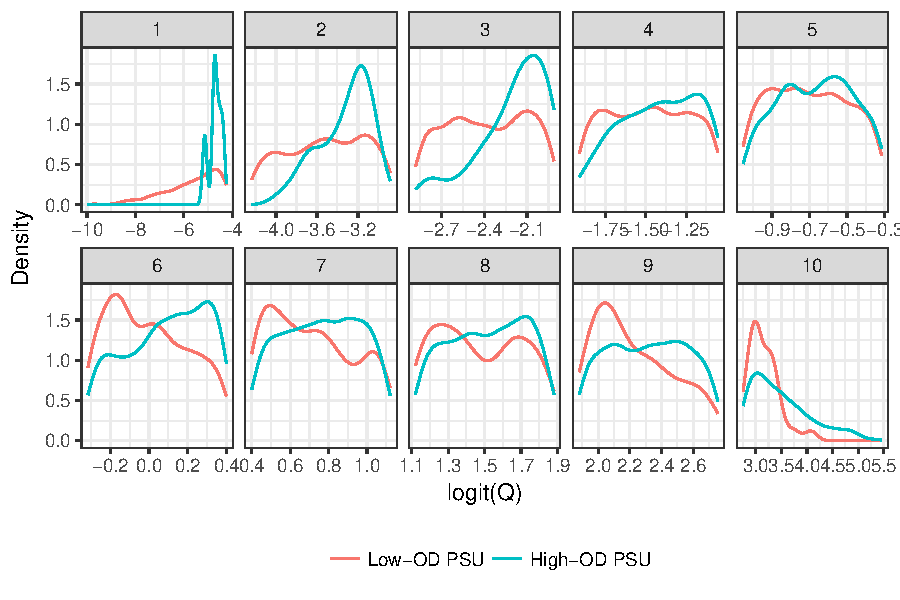
\includegraphics[scale=.75]{logit_q_density_by_strat.pdf}
	\caption{Density of logit($\widehat{Q}_j$) by stratum and OD status.}
	\label{fig:logit_q_dens}
\end{figure}

\begin{figure}
	\centering
	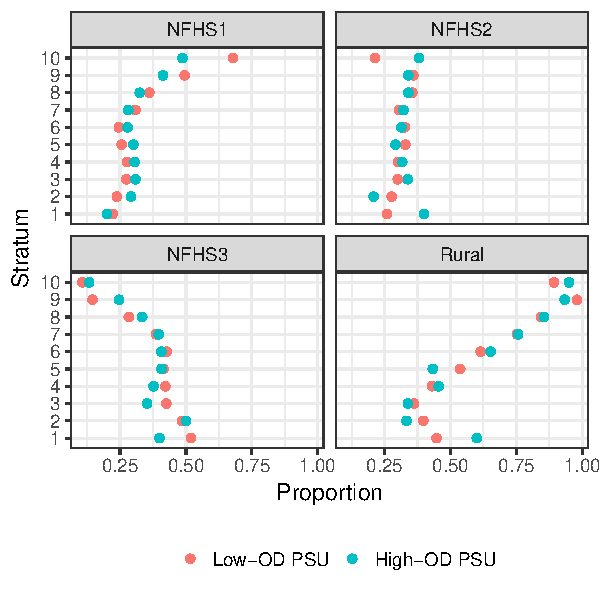
\includegraphics[scale=1]{cat_props_by_strat.pdf}
	\caption{Balance of survey rounds and rural residence within strata of logit($\widehat{Q}_j$).}
	\label{fig:cat_props}
\end{figure}

\begin{figure}
	\centering
	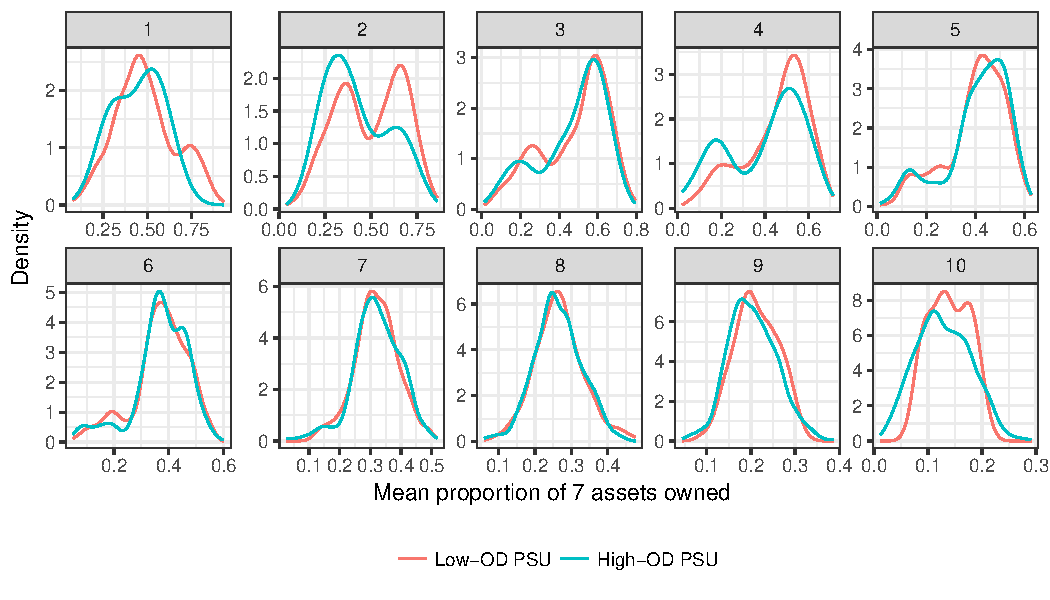
\includegraphics[scale=.7]{prop_assets_by_strat.pdf}
	\caption{Density of asset ownership by stratum and OD status.}
	\label{fig:ass_dens}
\end{figure}

\begin{figure}
	\centering
	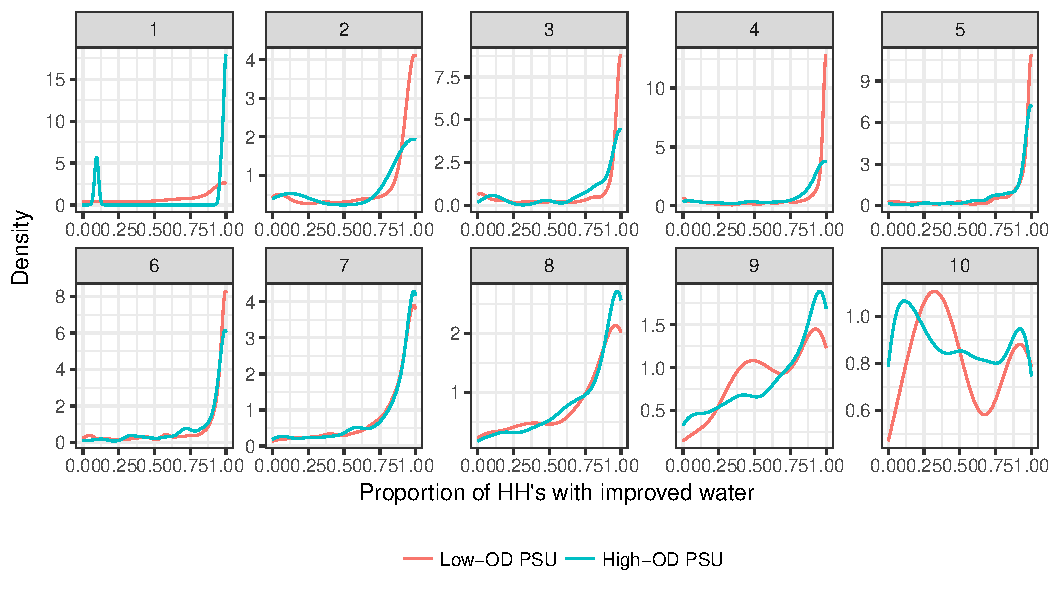
\includegraphics[scale=.7]{prop_water_by_strat.pdf}
	\caption{Density of proportion of households with improved water source by stratum and OD status.}
	\label{fig:wat_dens}
\end{figure}

\begin{figure}
	\centering
	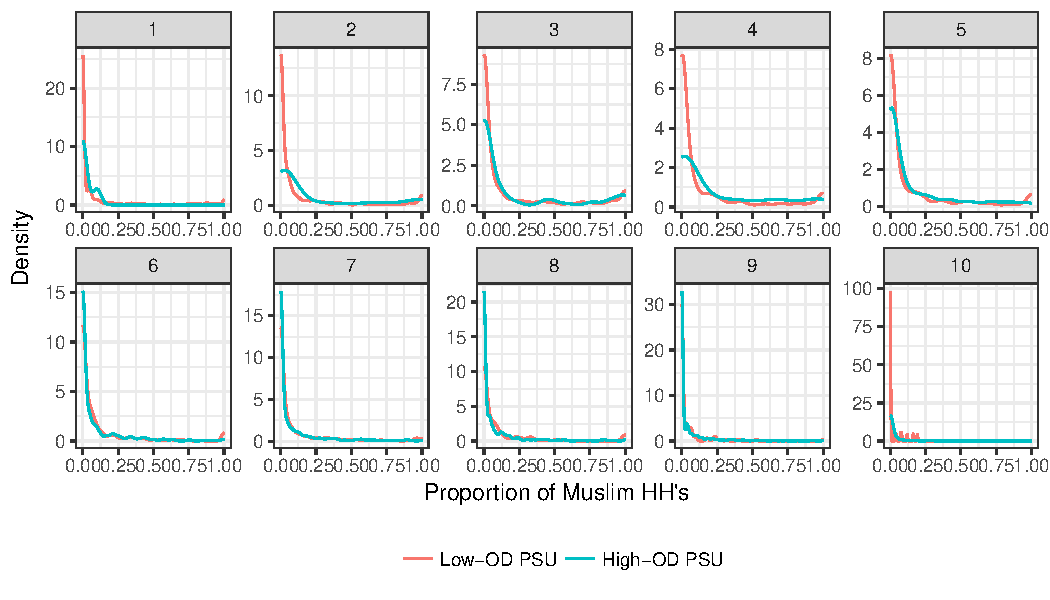
\includegraphics[scale=.7]{prop_muslim_by_strat.pdf}
	\caption{Density of proportion of Muslim households by stratum and OD status.}
	\label{fig:mus_dens}
\end{figure}

\begin{figure}
	\centering
	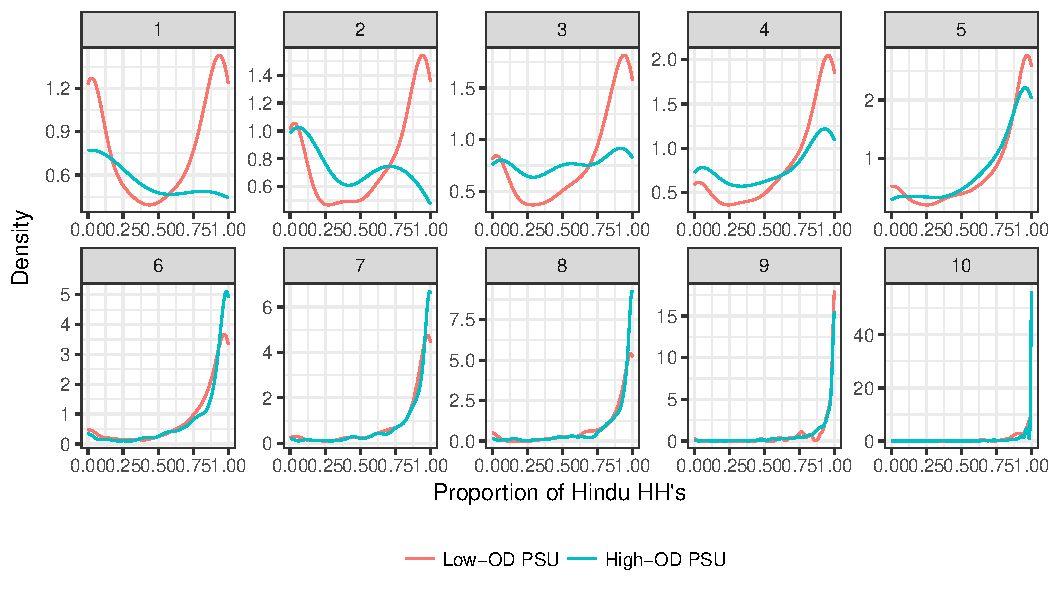
\includegraphics[scale=.7]{prop_hindu_by_strat.pdf}
	\caption{Density of proportion of Hindu households by stratum and OD status.}
	\label{fig:hin_dens}
\end{figure}

We now turn to modeling $q_1$ and $q_0$. We again use a hierarchical logistic regression model with household-level predictors and a neighborhood-level varying intercept. For $q_1$, we estimate the model
\begin{align*}
	\text{logit}(q_{1i}) &= \beta_0 + \beta_1 \mathbf{1}(NFHS2) + \beta_2 \mathbf{1}(NFHS3) + \\
	&\quad~ \beta_3 \mathbf{1}(rural_i) + \beta_4 assets_i + \beta_5 water_i + \beta_6 muslim_i + \beta_7 hindu_i + u_{j[i]} \\
	u_j &\sim N(0, \sigma_u^2),
\end{align*} 
where $i$ now indexes households and $j$ indexes neighborhoods. The predictor $assets_i$ is the proportion of the seven assets owned by household $i$, $water_i$ is an indicator for having an improved water source, and $muslim_i$ and $hindu_i$ are indicators for Muslim and Hindu households, respectively. We estimate logit($\widehat{q}_1$) using only the children in high-OD neighborhoods.

Following HR, we can identify the subpopulation that each child belongs to given these quantities. To identify subpopulation (AB), children ever-at-risk for living in households that practice OD, we stratify the estimated values logit($\widehat{q}_1$) into 10 strata. We then take the minimum observed value of logit($\widehat{q}_1$) among children in OD households and classify children in non-OD households whose logit($\widehat{q}_1$) is less than this minimum as belonging to subpopulation (C). All other children whose logit($\widehat{q}_1$) is above the minimum are considered part of subpopulation (AB).

We estimate logit($\widehat{q}_0$) using analogous modeling and stratification strategies, this time using only children in low-OD neighborhoods. We calculate the minimum value of logit($\widehat{q}_0$) among children in non-OD households and classify all children in low-OD neighborhoods with logit($\widehat{q}_0$) above this minimum as belonging to subpopulation (C). Figures \ref{fig:logit_q0} and \ref{fig:logit_q1} show the estimated values of logit($\widehat{q}_1$) and logit($\widehat{q}_0$) by household OD status.

\begin{figure}[h!]
	\centering
	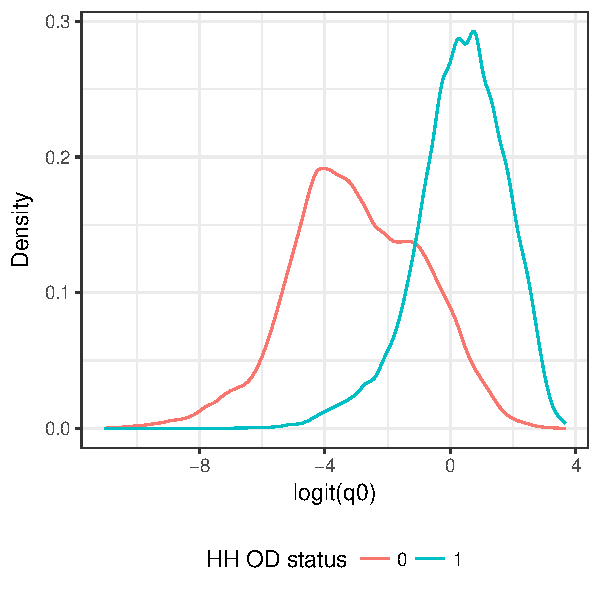
\includegraphics[scale=.7]{logit_q0.pdf}
	\caption{Density of logit($\widehat{q}_0$) for OD and non-OD households in low-OD neighborhoods.}
	\label{fig:logit_q0}
\end{figure}

\begin{figure}[h!]
	\centering
	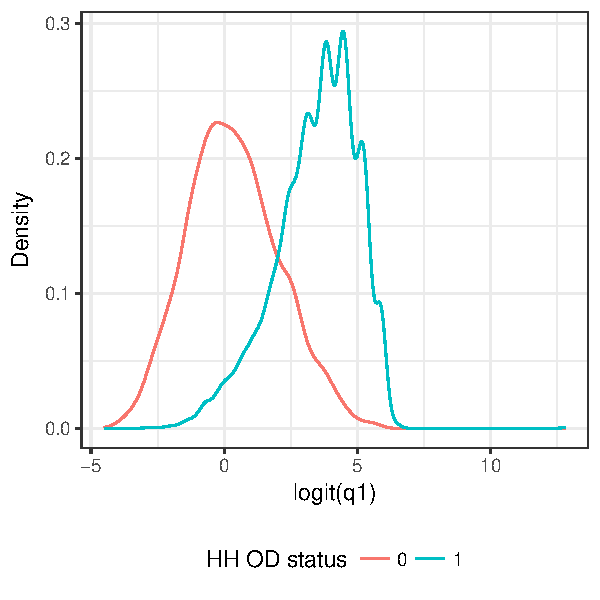
\includegraphics[scale=.7]{logit_q1.pdf}
	\caption{Density of logit($\widehat{q}_1$) for OD and non-OD households in high-OD neighborhoods.}
	\label{fig:logit_q1}
\end{figure}


\section{Limitations}\label{sec:lims}
One limitation of the present study is that we have ignored the clustering of children within households, thus implicitly treating children in the same community as independent. Children within the same household are likely to be more similar than children in different households, so if the data for a community has many children clustered in only a few households, they are less informative than they would be for a community with the same number of children with one child per household. However, 89\% of the children in our data belong to unique households and 81\% to unique mothers.

Our models do not take the state of residence into account due to computational constraints. However, the large differences in OD rates between states make this an important source of variation to account for. Careful consideration of how to best capture the relationship between states, neighborhoods, and survey rounds will yield more precise estimates.

We also do not know the geographic size of the PSUs. While the DHS manual tells us that urban PSUs are generally census enumeration blocks (roughly 150-200 households) and rural PSUs are villages of 500 or fewer households, there is likely to be variation in the geographic size and population density of the PSUs. In that case, our results are likely to be lower bounds, as the median sample size per PSU is 29 households (interquartile range 22 to 33). A recent study using both cross-national data from 172 countries and subnational data from Bangladesh suggests that the negative effects of neighborhood-level open defecation are magnified by high population density \citep{hathi2017}. However, an epidemiological study in Guatemala did not find that population density was an important determinant of intestinal infections or a strong effect modifier for household-level sanitation \citep{guatemala}, so evidence remains mixed.

\end{appendices}

\end{document}